\documentclass[tikz,border=2pt]{standalone}
\usepackage{times}
\usepackage{amsmath}
\usepackage{pgfplots}
\pgfplotsset{compat=1.16}
\begin{document}
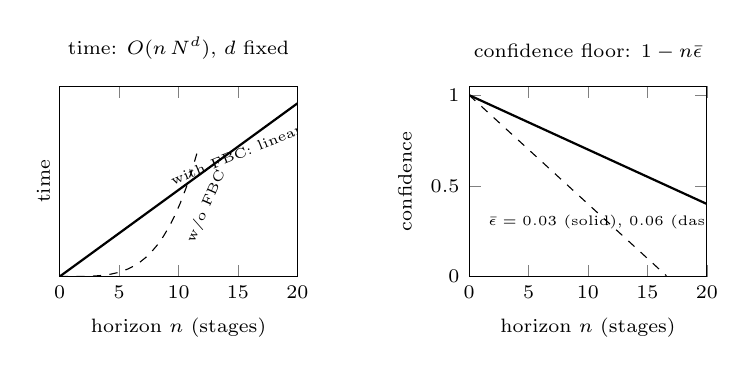
\begin{tikzpicture}
\begin{axis}[
  width=4.6cm, height=4.0cm,
  font=\scriptsize,
  xlabel={horizon $n$ (stages)},
  ylabel={time},
  ymin=0, ymax=22, xmin=0, xmax=20,
  ytick=\empty,
  title={\scriptsize time: $O(n\,N^{d})$, $d$ fixed},
]
\addplot[domain=0:20, thick] {x};
\addplot[domain=0:11.6, dashed] {0.0008*pow(x,4)};
\node[font=\tiny, anchor=west, rotate=22] at (axis cs:8.6,10.6) {with FBC: linear in $n$};
\node[font=\tiny, anchor=west, rotate=66] at (axis cs:10.7,3.0) {w/o FBC};
\end{axis}
\begin{scope}[xshift=5.2cm]
\begin{axis}[
  width=4.6cm, height=4.0cm,
  font=\scriptsize,
  xlabel={horizon $n$ (stages)},
  ylabel={confidence},
  ymin=0, ymax=1.05, xmin=0, xmax=20,
  title={\scriptsize confidence floor: $1-n\bar\epsilon$},
]
\addplot[domain=0:20, thick] {1-0.03*x};
\addplot[domain=0:16.6, dashed] {max(0,1-0.06*x)};
\node[font=\tiny, anchor=west] at (axis cs:0.8,0.30) {$\bar\epsilon=0.03$ (solid), $0.06$ (dashed)};
\end{axis}
\end{scope}
\end{tikzpicture}
\end{document}
